\documentclass[a4paper,11pt,liststotocnumbered,bibtotocnumbered]{scrartcl}
\usepackage[french]{babel}
\usepackage[utf8]{inputenc}
\usepackage[T1]{fontenc}
\usepackage{pst-all}
\usepackage{vanadin}
\usepackage{isotope}
\usepackage{longtable}
\usepackage{color}
\usepackage{amsmath}
\usepackage{units}
\usepackage{float}


\subject{TP~5 Physique nucléaire}
\title{Etude du flux du rayonnement cosmique}
\subtitle{Rayonnement cosmique}
\author{Mona Dentler, Sabine Engelhardt}
\publishers{Université Joseph Fourier, Grenoble}
\date{\today}

\begin{document}
 \nocite{poly}
 \pagestyle{empty}
 \begin{center}
  \makeatletter
   %\titlefont
  \@subject
  \vspace{2cm}

  \Huge
  Etude du flux du rayonnement cosmique\newline
  \vspace{1cm}
  \Large


  \@author
  \newline
  \@publishers


  \@date
  \makeatother
 \end{center}
 \vfill

 \begin{abstract}
  Le rayonnement cosmique qui bombarde en permanence l'atmosphère terrestre, consiste des particules de très haute énergie de l'origine solare, galactique ou intergalactique. Ces particules interagissent avec les particules de l'atmosphère et créent des particules secondaires de durée plus ou moins court. Au niveau de sol on peut détecter pour la plupart des muons.\\
  Dans cette TP nous mesurons le flux de muons crées par le rayon cosmique à l'aide de trois détecteurs de particules chargées. Ceux-ci sont monté une sur l'autre avec un certain distance pour permettre une mesure de co\"{\i}ncidence entre les détecteurs. Pour obtenir un bon résultat il faut premièrement calibré le système à l'aide des mesures préliminaires et deuxièment il faut calcule l'efficacité des détecteurs et les défauts peut-être par bruit mesuré.
 \end{abstract}
\newpage
 \pagestyle{scrheadings}
 \tableofcontents
\newpage

 \begin{section}{Le rayonnement cosmique}
  Les gerbes atmosphèriques sont créées quand le rayonnement cosmique arrive à l'atmosphère terrestre et les particules de très haute énergie interagissent avec les particules de l'atmosphère. A partir d'une particule primaire se forme beaucoup des particules secondaires. Le rayonnement cosmique se compose comme suivant:
   \begin{figure}[htb]
    \centering
    \begin{tabular}{lcr}
     Protons (noyeaux de Hydrogen) & $\simeq$ & 85~\%\\
     Particules $\alpha$ (nouyeaux d'Helium) & $\simeq$ & 12~\%\\
     Noyeaux avec Z $\geq 3$	& $\simeq$ & 2~\%\\ 
     Electrons, rayonnement $\gamma$	& $\simeq$ & 1~\%\\
    \end{tabular}\cite[S. 14]{burak}
   \end{figure}	

   \subsection{Gerbes électroniques}
    Les photons peuvent interagir en trois fa\c con pour créer des particules secondaires:
    \begin{enumerate}
     \item{Effet photoélectrique}
     \item{Effet Compton}
     \item{Annihilation électron-positon}
    \end{enumerate}
    Un photon d'énergie basse ne peut qu'integragir en effet photoélectrique et en effet Compton avec une particules de l'atmosphère, quand à un photons de très haute énergie qui peut créer un pair dans le cortège électronique d'un atome si l'énergie du photon est plus grande que la double énergie au repos d'un électron. Le positon et l'électron de la création d'un pair envoyent des photons secondaires par rayonnement continu de freinage.
    La création d'un pair électron-positon ne peut pas avoir lieu dans le vide, car là il n'y a pas avoir en même temps la conservation d'impulse et d'énergie. Donc les photons $\gamma$ peuvent traverser l'espace et ne déchaîne un gerbe que dans l'atmosphère terrestre.

    \begin{figurehere}
     \begin{minipage}{0.45\textwidth}
      \center 
     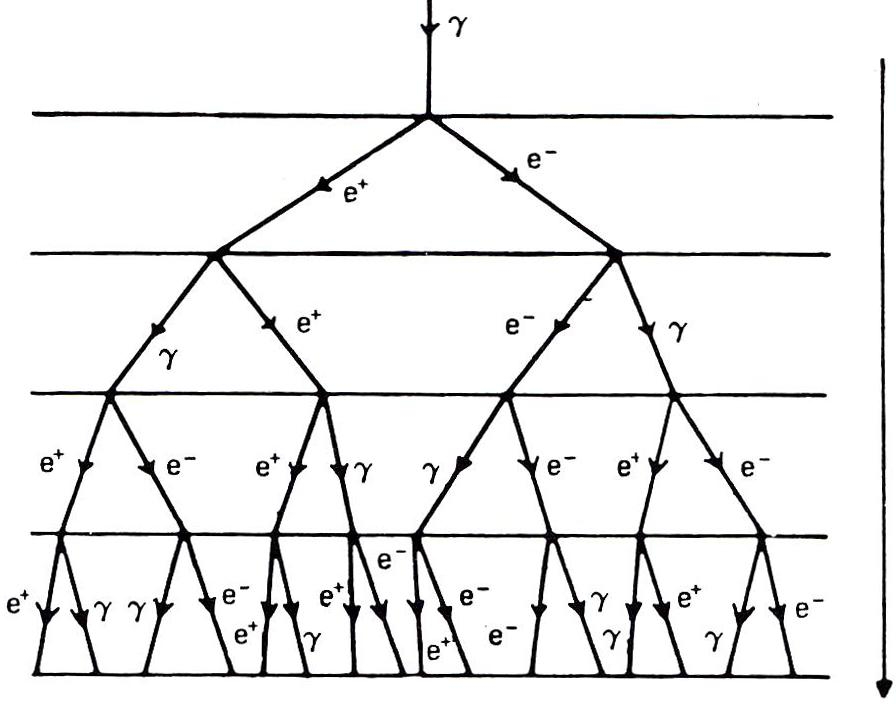
\includegraphics[width=\textwidth]{bilder/emschauer.jpg}   
     \caption{Modèle d'une gerbe électronique}   
     \label{fig:emschauer}  
     \end{minipage}
     \begin{minipage}{0.5\textwidth}
      Ce schéma \ref{fig:emschauer} montre le modèle d'une gerbe électronique crée par un photon $\gamma$. Un photon secondaire peut aussi générer un pair électron-positon. La gerbe s'arrête quand la particule genéré n'a pas l'énergie nécessaire pour créer un pair et le rayonnement continu de freinage ne peut non plus genérer des photons secondaire qui ont assez d'énergie pour créer un pair.
     \end{minipage}
    \end{figurehere}
 
  \subsection{Cascade hadronique}
   Les protons de très haute énergie ou les noyeaux lourds, appelés les hadrons, du rayonnement cosmique interagissent dans les couches supérieures de l'atmosphère avec les molécules de l'air. Pendant ce processus des particules secondaires en plupart des pions $\pi^+$, $\pi^-$ ou $\pi^0$ sont crées. 
   \begin{figure}[htb]
    \center
    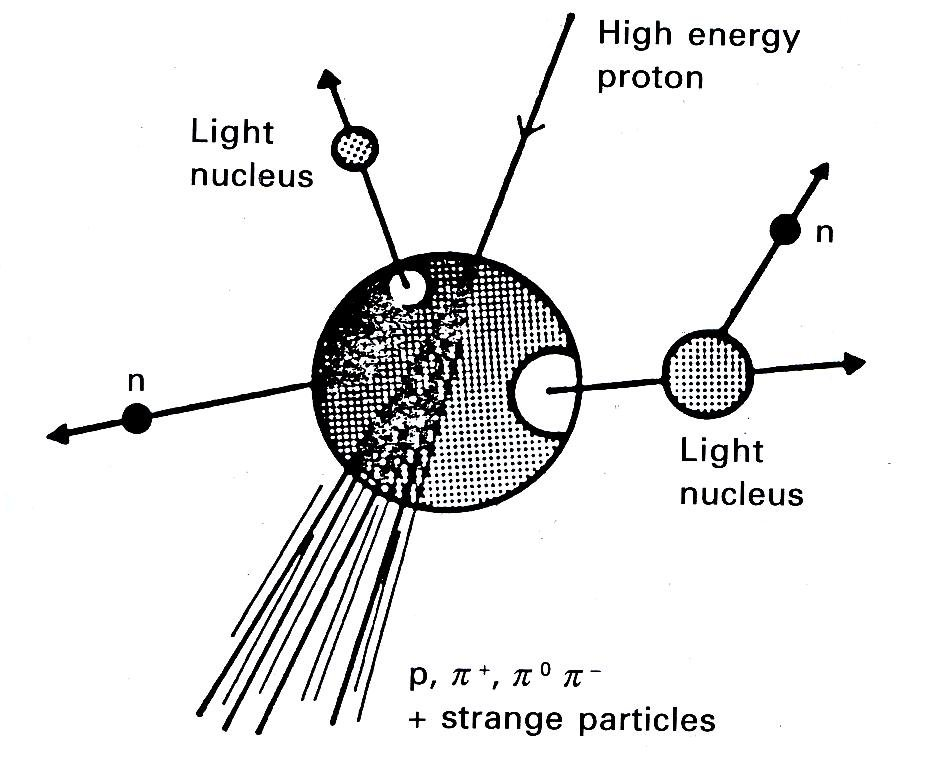
\includegraphics[width=0.6\textwidth]{bilder/03.jpg}
    \caption{Schéma de la réaction d'un proton de très haute énergie avec un noyeau de l'atmosphère}
    \cite[S.~133]{longair}
    \label{fig:preaktion}
   \end{figure}

   Pendant leur vol les pions se désintègre en muon
   \begin{equation*}
    \left.
    \begin{array}[]{lll}
     \pi^{+} & \rightarrow & \mu^{+} + \nu_{\mu}\\
     \pi^{-} & \rightarrow & \mu^{-} + \overline{\nu}_{\mu}\\	
    \end{array}
    \right\} \idx{Durée de vie moyenne: } \tau=\unit[2,551\cdot10^{-8}]{s}
    \left.
    \begin{array}[]{lll}
     \pi^{0} & \rightarrow & 2\gamma	
    \end{array}
    \right\} \tau=\unit[8,4\cdot10^{-17}]{s}
   \end{equation*}

   Les muons sont freinés par ionisation est se désintègre en positons, électrons, (anti)neutrinos muoniques et (anti)neutrinos électroniques. 

   \begin{equation*}
    \left.
    \begin{array}[]{lll}
     \mu^{+} & \rightarrow & \text{e}^{+} + \nu_{\text{e}} + \overline{\nu}_{\mu}\\
     \mu^{-} & \rightarrow & \text{e}^{-} + \overline{\nu}_{\text{e}} + \nu_{\mu}
    \end{array}
    \right\} \text{Durée de vie moyenne } \tau=\unit[2,2001\cdot10^{-6}]{s}
   \end{equation*}

   La plupart des particules secondaires est crées dans les couches supérieures de l'atmosphère par les hadrons. Les particules volent dans un disque vouté au sol. Cette voûte est causé par l'angle de diffusion différent des particules. .Les particules avec un angle de diffusion plus grand en un trajet plus longue jusqu'au sol. Seulement les muons sont detectés sur sol car ils ont une durée de vie relativement longue. 
   \begin{figure}[H]
    \center
     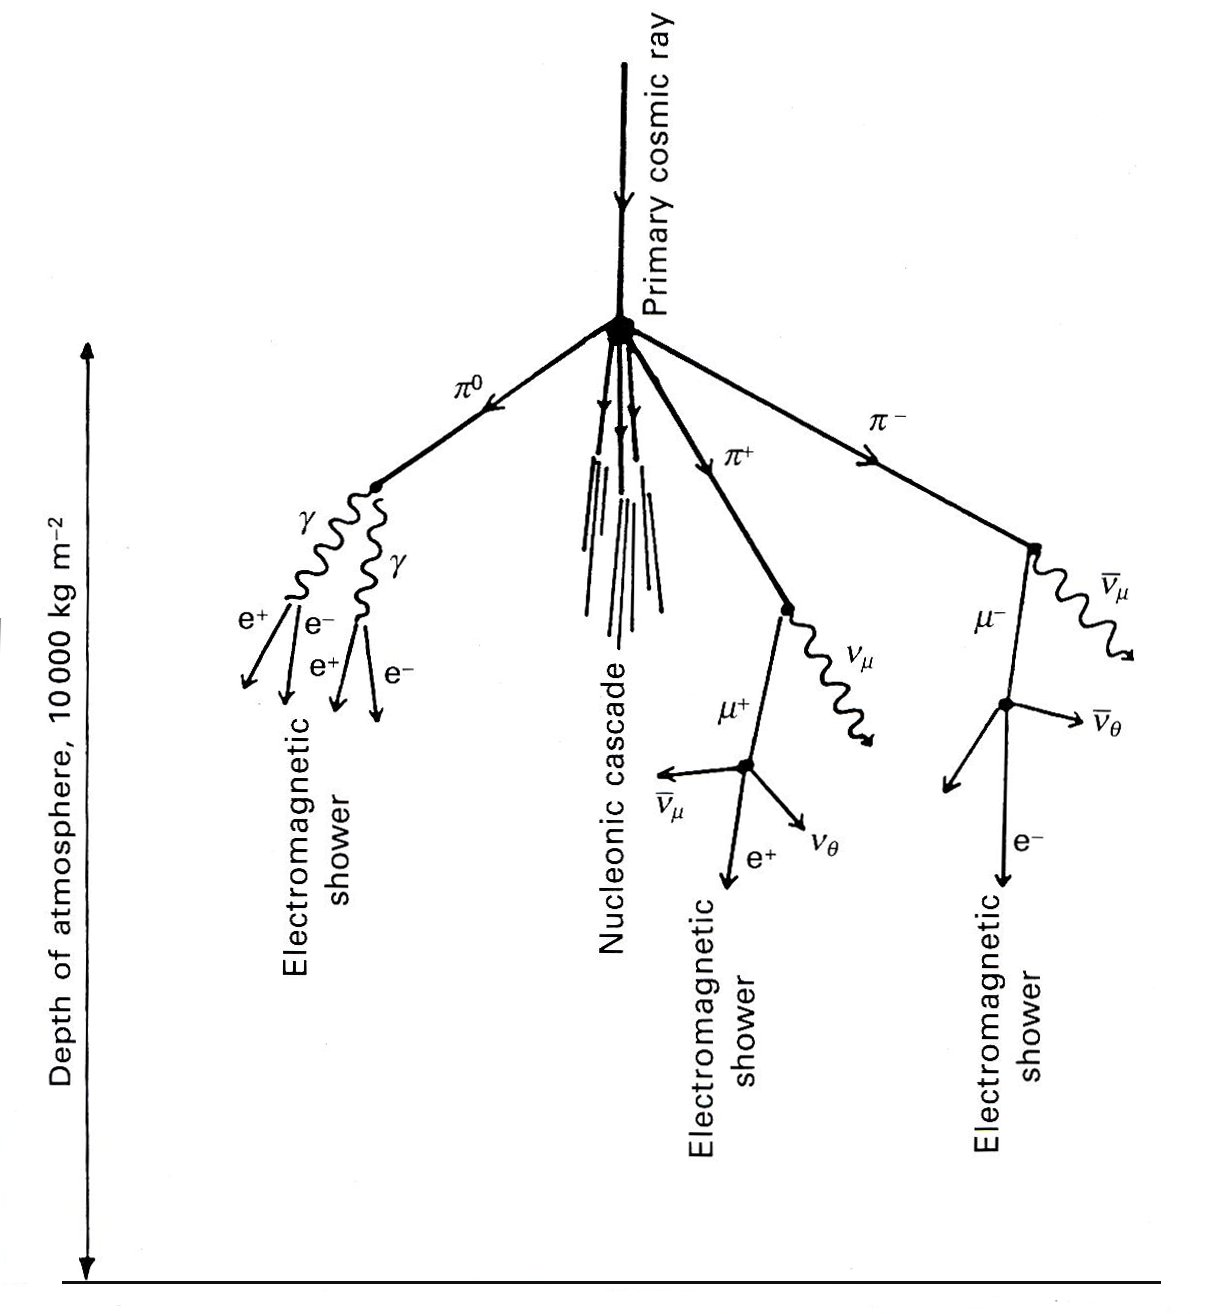
\includegraphics[width=0.7\textwidth]{bilder/hadronischer_schauer.jpg}
     \caption{Gerbe hadronique}
   \end{figure}
    
   Pour verifier que les muons arrivent au sol on peut faire un calcul. Un muon a une masse de repos $m_0=\unit[105,7]{\frac{MeV}{c^2}}$ et une durée de vie d'environ $\tau=\unit[2,2]{\mu s}$. La nombre des muons après un temps $t$ est donné part
   \begin{eqnarray*}
    n(t)=n_0\cdot\exp\left(-\frac{t}{\tau}\right)\\
   \end{eqnarray*}
   On considère un ensemble de muons produits à $l=\unit[10]{km}$ d'altitude et se dirigeant droite vers le sol. Un muon un une énergie cinétique moyenne $E_{cin}=\unit[2]{GeV}$.
   \paragraph{Calcul non-relativiste}
    Pour obtenie $t=l\cdot v$, il faut d'abord calculé la vitesse $v$ d'un muon.
    \begin{eqnarray*}
     E_{cin}=\frac{1}{2}m_0v^2\\
     v=\sqrt{\frac{2E_{cin}}{m_0}}=6,15c
    \end{eqnarray*}
    Donc les muons seraient plus vite que la lumière, ce qui n'est pas possible après Einstein.

   \paragraph{Calcul relativiste}
   Il faut de nouveau calculé la vitesse, mais cette fois relativistiquement, car on sait qu'un muon doit avoir une vitesse près de la vitesse de lumière $c$. 
   \begin{eqnarray*}
    E_{ges}\stackrel{Einstein}{=}mc^2=m_0\gamma c^2&=E_0\gamma &=E_0+E_{cin}\\
    \text{avec la masse relativiste }&m=m_0\gamma&\\
    \gamma=\left(1-\frac{v^2}{c^2}\right)^{-0,5}&=\frac{E_0+E_{cin}}{E_0}&\\
    \sqrt{1-\frac{v^2}{c^2}}&=\frac{E_0}{E_0+E_{cin}}&\\
    \Rightarrow v&=\sqrt{1-\left(\frac{E_0}{E_0+E_{cin}}\right)^2}c&\approx 0,999c
   \end{eqnarray*}
   Pour le temps de vol on trouve $t=l\cdot v=\unit[33,4]{ns}$.\\
   Alors $\frac{n(t)}{n_0}=\unit[98,5]{\%}$
 \end{section}

  
 \begin{section}{Préliminaire}
  \subsection{Préparation des photomultiplicateurs}
   \todo{ausführen}
   Pour obtenir une bonne mesure les signaux emettés des deux photomultiplicateurs doivent être précise. L'image suivant montre un bon signal d'un PMT en mesurant un photon $\gamma$. Il n' y a qu'un signal bien défini et à peine de bruit qui peut déranger le signal. Quand même il faut mettre un seuil (thresh) pour qu'on ne mesure que les vraies signaux.  
   \begin{center}
    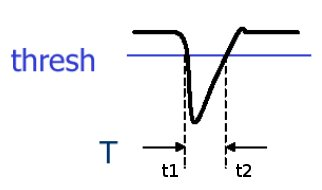
\includegraphics[width=0.5\textwidth]{bilder/pmtpuls.jpg}
   \end{center}
  \begin{tabular}{c|c|c|c}
      &temps de descente [ns]	&temps de montée [ns]	&amplitude$_{max}$ [mV]\\
    \hline
PMT 1	&	4,4	&	12,8	&	27,8	\\
PMT 2	&	5,6	&	8	&	29,2	\\
PMT 3	&	6,0	&	27,6	&	82,4	\\
	&	5,6	&	13,2	&	43,6	\\
   \end{tabular}
\newline

 Après l'analyse des signaux nous avons mis le seuil pour le PMT 1 à \unit[19]{mV} et pour le PMT 2 à \unit[25]{mV} et pour le PMT 3 à \unit[24]{mV}. Nous avons vu que les PMT ont des signaux similaire, \c ca veut dire qu'ils transforment le signal d'un $\gamma$ de la même fa\c con.

  \end{subsubsection}

  \subsection{Réglage de la co\"{\i}ncidence}
   \todo{neue Daten einsetzen}\\

   \subsubsection{Générer un signal logique}
    Le module de co\"{\i}ncidences ne peut qu'évaluer des signaux logique, alors il faut générer un signal logique du signal analytique des PMT. Nous avons utilisé deux discriminateurs pour réussir à le faire. De fa\c con à pas obtenir des cascades des signaux à partir d'un seul signal, il faut ensuite mettre le seuil découvrit et mettre la largeur des créneaux à environ \unit[600]{ns}. Les signaux des deux PMT sont observés à l'oscilloscope aous l'aspect s'ils sont en co\"{\i}ncidence.
   
  
   \subsubsection{Comptage}
    Après avoir observer les signaux en co\"{\i}ncidence sur l'écran de l'oscilloscope (malheuresement nous n'avons pas réussi à faire un screenshot) nous avons relié les sorties des deux discriminateurs à un module de co\"{\i}ncidence. Le sortie de celui est connecté à l'echelle de comptage. Une mesure de \unit[10]{s} a montré que les signaux sont comptés.
   
   
   \subsubsection{Première mesure}

 \begin{tabular}{c|c|c|c|c}
   	&	PMT 1	&	PMT 2	&	PMT 3	&	Co\"{\i}ncidences 1 $\leftrightarrow$ 2	\\ \hline
1	&	123587	&	10072	&	4081	&	519	\\
2	&	123224	&	9877	&	4027	&	486	\\
3	&	122707	&	10039	&	4081	&	547	\\
4	&	122949	&	10059	&	4135	&	525	\\
5	&	123761	&	10036	&	4178	&	555	\\ \hline
moyenne M	&	123245,6	&	10016,6	&	4100,4	&	526,4	\\
$\sqrt M$	&	351,06	&	100,08	&	64,03	&	22,94	\\
écart type $\sigma$	&	436,10	&	79,42	&	57,79 &	27,07	\\ \hline
	&	PMT 1	&	PMT 2	&	PMT 3	&	Co\"{\i}ncidences 1 $\leftrightarrow$ 3	\\ \hline
1	&	124235	&	10032	&	4093	&	292	\\
2	&	122680	&	9910	&	4156	&	307	\\
3	&	123496	&	9940	&	4016	&	304	\\
4	&	123054	&	9806	&	4019	&	282	\\
5	&	122082	&	10011	&	4150	&	320	\\ \hline
moyenne M	&	123109,4	&	9939,8	&	4086,8	&	301	\\
$\sqrt M$	&	350,87	&	99,70	&	63,93	&	17,35	\\
écart type $\sigma$	&	815,39	&	89,95	&	67,88	&	14,56	\\
\end{tabular}

   \subsubsection{Interprétation} 
    Nous suposse que les dates sont decrit par la distribution de Poisson:
    \begin{equation*}
     P_{\mu}(n)=\frac{\mu^n}{n!}\cdot e^{-{\mu}}
    \end{equation*}
    Avec la moyenne $\mu$ et le nombre de fois $n$. On trouve pour $lim \; n {\rightarrow}  \infty$ que $\bar{n}$, la moyenne experimentale tend vers $\mu$ et l'écart type $\sigma$ vers $\sqrt{\mu}$:
    \begin{equation*}
     \bar{n}=\sum_{n=0}^{\infty} n \cdot P_{\mu}(n)=e^{-{\mu}}\sum_{n=1}^{\infty}\frac{\mu^n}{(n-1)!}=\mu \cdot  e^{-{\mu}}\sum_{k=0}^{\infty}\frac{\mu^k}{(k)!}=\mu \cdot e^{-{\mu}}\cdot  e^{{\mu}}=\mu
    \end{equation*}

    \begin{equation*}
     \begin{split}
      \sigma^2=\overline{(n-\bar{n}\,)^2}=\overline{n(n-1)}+\bar{n}-{\bar{n}}^2=\sum_{n=0} ^{N} n (n-1)\cdot P_{\mu}(n)+\mu -\mu^2=\\
      e^{-{\mu}}\sum_{n=2}^{\infty}\frac{\mu^n}{(n-2)!}+\mu -\mu^2=\mu^2+ \mu -\mu^2=\mu
     \end{split}
    \end{equation*}
    L'écart type de nos dates est dans les limites de $\sqrt{\mu}$ ce qui dit que les nombres mesurés sont bien. Il y a des petites différences qui peut être expliqué par le fait que plus des désintégration ou plus de bruit étaient mesuré.
   \subsubsection{Bruit}
Comme l'installation de la manip est bon, il se pose maintenant la question comment
savoir que les coïncidences mesurés ne sont pas des résultats des bruit. C'est pourquoi on retard un signal et compare \c ca avec un autre signal non retardé. \c Ca on fait en cause des bruits apparaissent aléatoirement et ne sont pas corrélés à les signals vrais, \c ca veut dire qu'en moyenne il y a le même nombre des co\"{i}ncidences entre le bruit d'une part et le signal retardé ou le signal non retardé  d'autre part. Au  contraire le vrais signals sont forcément corrélés donc on ne va plus messurer des co\"{i}ncidences entre les signal vrais.
\begin{figure*}[h]
   \begin{minipage}[H]{0.5\textwidth}
        \centering
	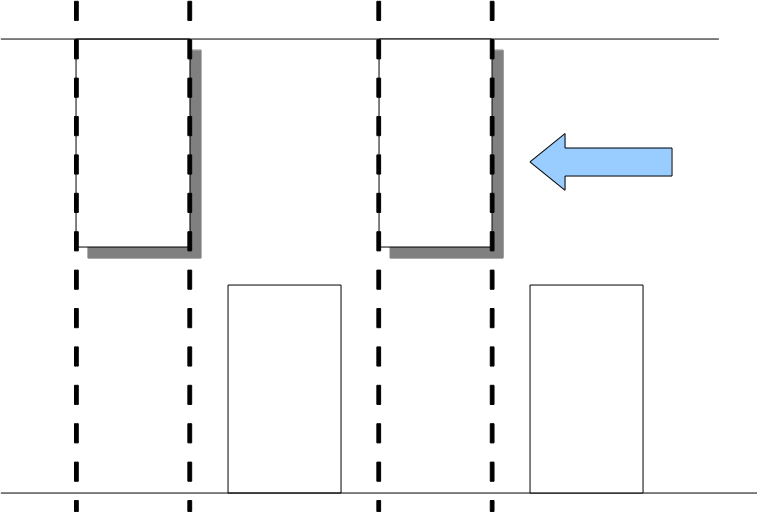
\includegraphics[width=0.5\textwidth]{bilder/retard.png}
        \caption{signal et signal retardé }
   \end{minipage}
   \hfill
   \begin{minipage}[H]{0.5\textwidth}
        \centering
       	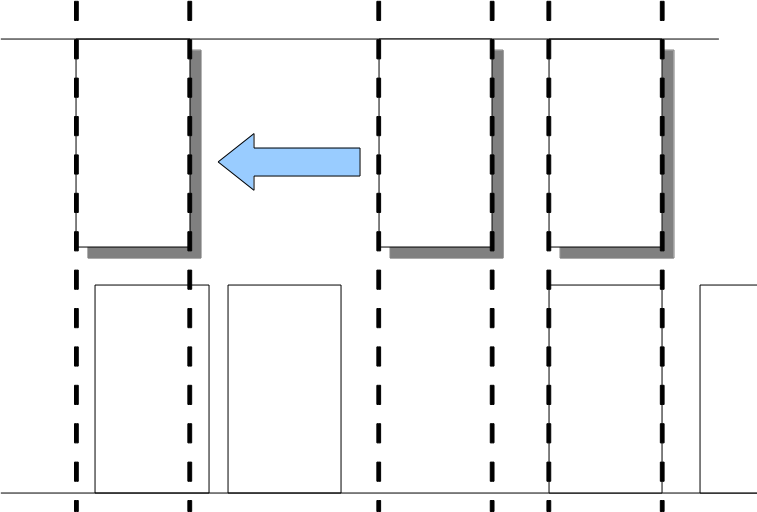
\includegraphics[width=0.5\textwidth]{bilder/retard2.png}
        \caption{signal et signal bruit retardé}
   \end{minipage}
   \end{figure*}
   \newline

  \begin{tabular}{c|c|c|c|c|c}
Co\"{\i}ncidences:	&	1 $\leftrightarrow$ 2 retardé	&	2 $\leftrightarrow$ 3 retardé	&	3 $\leftrightarrow$ 2 retardé	&	3 $\leftrightarrow$ 1 retardé	\\ \hline	

temps:	\unit[10]{s} &	0	&	0	&	0	&	0	\\
	&	0	&	0	&	0	&	0	\\
	&	0	&	0	&	0	&	0	\\
	&	0	&	0	&	0	&	0	\\ \hline
temps: \unit[100]{s}	&	1	&	0	&	0	&	0	\\
\end{tabular}
\newline
Les messures affichent qu' on peut néglige les co\"{i}ncidences fortunes.
 \end{section}


 \begin{section}{Mesure}
\begin{subsection}{Comptage avec deux photomultiplicateurs}
  \begin{tabular}{c|c|c|c}
Co\"{\i}ncidences	&	 1 $\leftrightarrow$ 2	&	2 $\leftrightarrow$ 3	&	 1 $\leftrightarrow$ 3	\\ \hline
1	&	1750	&	1661	&	991	\\
2	&	1783	&	1686	&	961	\\
3	&	1758	&	1695	&	968	\\
4	&	1822	&	1674	&	975	\\ \hline
moyenne M	&	1778,25	&	1679	&	973,75	\\
$\sqrt M$	&	42,17	&	40,98	&	31,20	\\
écart type $\sigma$	&	32,38	&	14,76	&	12,84	\\
\end{tabular}
\end{subsection}
\begin{subsection}{Comptage avec les trois photomultiplicateurs}
\begin{tabular}{c|c|c|c|c}
Co\"{\i}ncidences	&	 1 $\leftrightarrow$ 2	&	 2 $\leftrightarrow$ 3	&	 1 $\leftrightarrow$ 3	&	 $\leftrightarrow$ 2 $\leftrightarrow$ 3	\\ \hline
temps: 100 s	&	1622	&	1488	&	843	&	813	\\
	&	1598	&	1552	&	871	&	834	\\
	&	1622	&	1542	&	893	&	864	\\
	&	1633	&	1594	&	910	&	883	\\
	&	1657	&	1562	&	909	&	867	\\ \hline
moyenne M	&	1627,5	&	1562,5	&	895,75	&	862,00	\\
$\sqrt M$	&	40,34	&	39,53	&	29,93	&	29,36	\\
écart type $\sigma$	&	24,50	&	22,53	&	18,25	&	20,45	\\ \hline
temps: 1000s	&	16506	&	15846	&	9054	&	8770	\\
\end{tabular}
\end{subsection}
 \end{section}


 \begin{section}{Conclusion}
  
 \end{section}
 
 \begin{appendix}
  \bibliographystyle{unsrt}
  \bibliography{literatur}  

  \listoffigures  
 \end{appendix}

\end{document}

